\documentclass[12pt, a4paper]{article}
\usepackage[utf8]{inputenc}
\usepackage{lmodern}
\usepackage[english]{babel}
\usepackage[L7x]{fontenc}
\usepackage{url}
\usepackage{minted}
\usepackage{float}
\usepackage{indentfirst}
\usepackage{tikz}
\usepackage{graphicx} 

\def\checkmark{\tikz\fill[scale=0.4](0,.35) -- (.25,0) -- (1,.7) -- (.25,.15) -- cycle;} 
\graphicspath{ {./images/} }

\begin{document}
\pagenumbering{gobble}
\begin{titlepage}
\begin{center}
\vspace*{1cm}

\textbf{Vilnius University}

\textbf{Faculty of Mathematics and Informatics}

\textbf{Informatics}

\vfill

\textbf{Numerical investigation of Reinforcement Learning algorithms}

\vspace{0.5cm}

\textbf{Skatinamojo mokymo algoritmų palyginimas}

\vspace{0.5cm}

Project work

\vfill

\begin{tabular}{p{8cm} p{6cm}}
By: & Arnoldas Čiplys\\
Supervisor: & asist. dr. Linas Petkevičius\\
\end{tabular}

\vfill

Vilnius - 2021

\end{center}
\end{titlepage}
\newpage
\pagenumbering{arabic}
\setcounter{page}{2}
\setcounter{tocdepth}{3}
\setcounter{secnumdepth}{5}

\tableofcontents

\newpage

\section*{Introduction}
\addcontentsline{toc}{section}{Introduction}

\subsection*{Background}

%\verb||

Reinforcement learning (abbreviated as RL) is an area of machine learning that learns to maximize reward by not being told what actions to take,
but by using trial and error to discover which actions yield the most reward.
Usage of reinforcement learning for creating AI is very advantageous in various tasks, since it can learn without any training data and just by exploring environment itself,
just like humans or animals learn.

There are many different reinforcement learning algorithms created for many different purposes and one of the most asked questions is which algorithm to use.
In this thesis, the investigation by the author is done by analyzing how different algorithms perform in simple game environments comparing their training speed and performance results to try to answer that question.

\subsection*{Purpose}

The goal of this topic is to compare different reinforcement learning algorithms by trying to find the best algorithm for simple computer game environments.

\subsection*{Objectives} 
Goals for this topic:
\begin{itemize}
  \item Choose and prepare training environment for agents.
  \item Choose few different popular RL algorithms to be compared.
  \item Perform experiments using chosen algorithms.
  \item Compare experiment results and draw conclusions.
\end{itemize}

\newpage

\section{Reinforcement Learning}

Reinforcement learning is one of the main machine learning (ML) branches alongside supervised learning and unsupervised learning. The simplest RL model consists from agent, which observes environment and makes decisions, and environment, which takes input, changes state and gives reward to the agent \cite{Sutton1998}, see Figure \ref{rlexample}.

\begin{figure}[h]
    \centering
    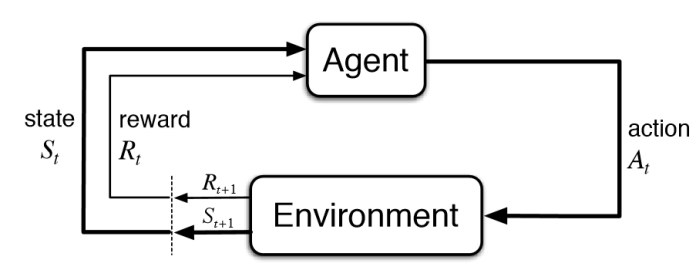
\includegraphics[width=.8\linewidth]{rl.jpg}
    \caption{Simplified RL example, taken from \cite{Sutton1998}}
    \label{rlexample}
\end{figure}

\subsection{Action and observation space}

To interact with the environment, agent has to take action. This action type can vary depending on chosen environment, however, it falls into 1 of these 2 categories or their combinations: discrete and continuous. Discrete action space is arguably the most used action space, where each action is an integer from finite natural numbers range, where each number represents specific action. Continuous actions space is a real number/vector, rather than a discrete choice of many options \cite{kanervisto:2020}.

Observation space classification is identical to action space, however, it represents not action, which agent takes, but observation, which agent receives after taking action.

\newpage

\section{Methodology}

Environment, algorithms and RL library choices will be described in this section.

\subsection{Environment}

This subsection describes everything about selected environments and how they were chosen.

\subsubsection{Environment selection}

In order to compare different RL algorithms, it is necessary for them to have a common environment to train on. Luckily, due to RL popularity, many libraries already exist that takes care of it.

Some of the most popular game environment libraries:
\begin{itemize}
  \item DeepMind Lab\footnote{https://github.com/deepmind/lab} \cite{beattie:2016} - 3D learning environment based on Quake III Arena\footnote{https://github.com/id-Software/Quake-III-Arena} via ioquake3\footnote{https://github.com/ioquake/ioq3}. It provides challenging 3D navigation and puzzle-solving tasks for learning agents. It is frequently updated, however, it only works on Linux systems and documentation is a bit lacking.
  \item OpenAI Gym\footnote{https://gym.openai.com} \cite{1606.01540} - toolkit specifically designed for comparing RL algorithms. It is frequently updated, has amazing documentation and is heavily used by the community. Additionally, there is a big range of environments to choose from, official and community written.
  \item OpenSpiel\footnote{https://github.com/deepmind/open\_spiel} \cite{LanctotEtAl2019OpenSpiel} - collection of environments for research in general RL and search/planning in games. Consists mostly of table and cards games, which require 2 or more players. Similar to DeepMind Lab, it only works on Linux systems and documentation and examples are limited.
\end{itemize}

For this task OpenAI Gym was chosen for its usage simplicity and amazing community support.
Additionally, to have agents training converge in a reasonable amount of time and prevent luck coming into play, environment should be simple enough, which quickly rules out other choices.

\subsubsection{OpenAI Gym toolkit}

OpenAI Gym is created by OpenAI\footnote{AI research company. https://openai.com/} as a tool to compare and implement different algorithms to use in their already created various environments. It is open source library written purely in Python. At the core of it is interface \verb|gym.Env|, which is common between all implemented environments and additionally allows users to create their own custom environments. Its core methods, which are used to train agents, are:

\begin{itemize}
  \item \verb|step(self, action) -> observation, reward, done, info| - environment step method, which takes action from agent and returns observation about new environment state, gained reward, whether environment episode is done and other additional info. 
  \item \verb|reset(self) -> observation| - resets environment to fresh state for new episode and returns initial observations.
\end{itemize}

\paragraph{Environment}\mbox{}\\

Environments should not be overly complicated to allow agents to converge more quickly. For better representation of RL problems, 2 different environments are selected: with discrete and continuous actions spaces, since action space is very important part in agent training. Selected environments are 2 classic control theory problems from RL literature: CartPole and Pendulum, see Figure \ref{CartpolePendulumExample}.

\subparagraph{CartPole environment}\mbox{}\\

CartPole is an environment, where a pole is attached by an un-actuated joint to a cart, which moves along a frictionless track. The pendulum starts upright, and the goal is to prevent it from falling over. A reward is given for every timestep that the pole remains upright.\footnote{https://gym.openai.com/envs/CartPole-v1} This environment corresponds to the version of the cart-pole problem described by Barto, Sutton and Anderson \cite{6313077}.

This environment have 4 observation variables: cart position, cart velocity, pole angle and pole angular velocity, and 2 possible discrete actions: push cart to the left or to the right. To make every episode unique, starting observations are selected randomly in specific range.

\subparagraph{Pendulum environment}\mbox{}\\

Inverted pendulum swingup problem is a classic problem in the control literature. In this version pendulum starts in random position and the goal is to swing it up and keep it upright.\footnote{https://gym.openai.com/envs/Pendulum-v0} 

This environment have 3 observation variables: sin and cos of the angle to represent rotation of the pendulum and angular velocity. It only has 1 action variable for the amount of force on the pendulum, which is real number instead of integer, meaning this environment has continuous action space.

\begin{figure}[H]
    \centering
    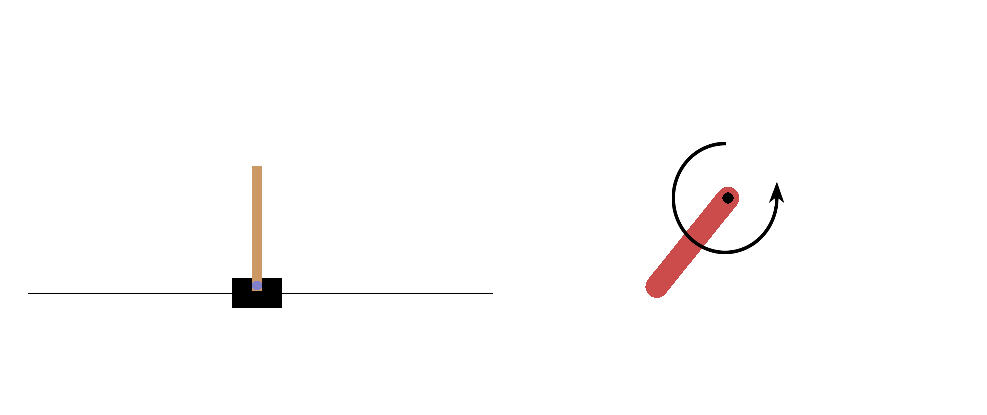
\includegraphics[width=.8\linewidth]{env-examples.png}
    \caption{CartPole (left) and Pendulum (right) environments example}
    \label{CartpolePendulumExample}
\end{figure}

\subsection{Reinforcement learning library}

This subsection describes everything about selected reinforcement learning library and how it was chosen.

\subsubsection{Reinforcement learning library selection}

RL is a very popular area for many ML related research nowadays, so, naturally, there are a lot of different implementations for many popular algorithms. Often these implementations get grouped into RL libraries, which have its own advantages and disadvantages. When choosing RL library, you have to weight which factors are more important for you: programming language, documentation and tutorials, regular updates and active community, compatibility with other libraries, which RL algorithms are implemented and etc.

Some of the most popular and well known RL libraries:
\begin{itemize}
  \item KerasRL\footnote{https://github.com/keras-rl/keras-rl} \cite{plappert2016kerasrl} - RL library built with Keras\footnote{Deep learning API written in Python, which focuses on enabling fast experimentation.}. It is very easy to start to use as there are simple documented examples to show its usage, however, even though it's possible to add your agent, implemented algorithm list is very limited and library had its last stable release in 2018, so it hasn't been updated lately.
  \item OpenAI Baselines\footnote{https://github.com/openai/baselines} \cite{baselines} - RL library made by OpenAI to be used for OpenAI Gym. Even though it implements latest state of the art algorithms, everything else is a bit lacking. Poor documentation, no commented code, difficult to modify or add custom agents/environments.
  \item Stable Baselines\footnote{https://github.com/hill-a/stable-baselines} \cite{stable-baselines} - RL library, which was forked from OpenAI Baselines repository and updated by the community. It still retains all the advantages of OpenAI Baselines and adds more customability and documentation.
  \item Tensorforce\footnote{https://github.com/tensorforce/tensorforce} \cite{tensorforce} - Tensorflow library for applied RL. Implements most of the well known algorithms and supports most of the environment libraries, however, documentation and examples does not go deep into it.
\end{itemize}

Stable Baselines was chosen for its great OpenAI Gym integration, ease to start and big implemented algorithm list. Additionally, TensorBoard support greatly helps with data storing, viewing and parsing.

\subsubsection{Stable Baselines library}

Stable Baselines \cite{stable-baselines} is a set of improved implementations of reinforcement learning algorithms based on OpenAI Baselines \cite{baselines}. This library implements most of the researched modern algorithms, however, 2 of them, GAIL (or Generative Adversarial Imitation Learning) \cite{ho:2016} and HER (or Hindsight Experience Replay) \cite{andrychowicz:2017}, requires additional previously trained data, usually done by other algorithms. For this reason they will not be compared alongside others.

\paragraph{Policy}\mbox{}\\

Stable Baselines have a list of already implemented policies, that could be used in each of algorithms. To make things simple, single common policy was chosen to be used for every agent. Selected policy is MLP Policy, which implements actor critic, using an MLP\footnote{Class of feedforward artificial neural network.} (2 layers of 64).

\paragraph{Algorithms}\mbox{}\\

All the algorithms, that will be used in this experiment and their quick descriptions:

\subparagraph{A2C}\mbox{}\\

Algorithm A2C (or Advantage Actor Critic) \cite{mnih:2016} is a synchronous, deterministic variant of Asynchronous Advantage Actor Critic (A3C). It uses multiple workers to avoid the use of a replay buffer.

\subparagraph{ACER}\mbox{}\\

Algorithm ACER (or Sample Efficient Actor-Critic with Experience Replay) \cite{wang:2016} is a combination of several other algorithm ideas: uses multiple workers like A2C \cite{mnih:2016}, implements replay buffer like DQN \cite{mnih:2013} and uses Retrace \cite{munos:2016} for Q-value estimation, importance sampling and a trust region.

\subparagraph{ACKTR}\mbox{}\\

Algorithm ACKTR (or Actor Critic using Kronecker-Factored Trust Region) \cite{wu:2017} was developed by researchers at the University of Toronto and New York University, which combines 3 distinct techniques: actor-critic methods \cite{mnih:2016}, trust region optimization \cite{schulman:2015} for more consistent improvement and distributed\footnote{https://jimmylba.github.io/papers/nsync.pdf} Kronecker factorization \cite{grosse:2016} to improve sample efficiency and scalability.

\subparagraph{DDPG}\mbox{}\\

DDPG (or Deep Deterministic Policy Gradient) \cite{lillicrap:2015} is an algorithm which concurrently learns a Q-function and a policy. It uses off-policy data and the Bellman equation to learn the Q-function, and then uses that Q-function to learn the policy.

\subparagraph{DQN}\mbox{}\\

Algorithm DQN (or Deep Q-Network) \cite{mnih:2013} combines Q-Learning with deep neural networks by approximating a state-value function in a Q-Learning framework with a neural network.

\subparagraph{PPO}\mbox{}\\

Algorithm PPO (or Proximal Policy Optimization) \cite{schulman:2017} combines ideas from A2C \cite{mnih:2016} (having multiple workers) and TRPO \cite{schulman:2015} (it uses a trust region to improve the actor).

\subparagraph{SAC}\mbox{}\\

Algorithm SAC (or Soft Actor Critic) \cite{haarnoja:2018} optimizes a stochastic policy in an off-policy way, forming a bridge between stochastic policy optimization and DDPG-style approaches.

\subparagraph{TD3}\mbox{}\\

Algorithm TD3 (or Twin Delayed DDPG) \cite{fujimoto:2018} is a direct successor of DDPG \cite{lillicrap:2015} and improves it using three major tricks: clipped double Q-Learning, delayed policy update and target policy smoothing. 

\subparagraph{TRPO}\mbox{}\\

Algorithm TRPO (or Trust Region Policy Optimization) \cite{schulman:2015} updates policies by taking the largest step possible to improve performance, while satisfying a special constraint on how close the new and old policies are allowed to be.

\paragraph{Algorithm action space}\mbox{}\\

Algorithm implementations heavily depend on environment action space for its training and some of the algorithms are specifically designed for only one type of action space, therefore not all algorithms in Stable Baselines have been implemented for both actions spaces. See Table \ref{AlgorithmActionSpacesTable} to see what actions does each algorithm support.

\begin{table}[H]
\centering
\begin{tabular}{|l|c|c|} 
\hline
Algorithm & \multicolumn{1}{l|}{Discrete} & \multicolumn{1}{l|}{Continuous}  \\ 
\hline
A2C       & $\checkmark$                    & $\checkmark$                        \\
ACER      & $\checkmark$                    & $\times$                            \\
ACKTR     & $\checkmark$                    & $\checkmark$                        \\
DDPG      & $\times$                        & $\checkmark$                        \\
DQN       & $\checkmark$                    & $\times$                            \\
PPO       & $\checkmark$                    & $\checkmark$                        \\
SAC       & $\times$                        & $\checkmark$                        \\
TD3       & $\times$                        & $\checkmark$                        \\
TRPO      & $\checkmark$                    & $\checkmark$                        \\
\hline
\end{tabular}
\caption{Stable Baselines algorithm action space support}
\label{AlgorithmActionSpacesTable}
\end{table}

\paragraph{Hyperparameters}\mbox{}\\

Default hyperparameter values, that were set by Stable Baselines authors for each algorithm, will be used in this experiment. Exact values can be found on Stable Baselines documentation\footnote{https://stable-baselines.readthedocs.io/en/master/index.html}.

\paragraph{TensorBoard}\mbox{}\\

TensorBoard\footnote{https://www.tensorflow.org/tensorboard} provides data visualization and management for machine learning experimentation. Stable Baselines have TensorBoard integration\footnote{https://stable-baselines.readthedocs.io/en/master/guide/tensorboard.html}, which will help to manage trained data.

\section{Experiments}

This section contains everything about experiments and their results.

\subsection{Experiments environment specifications}

Experiments were done using Ryzen 5 3600 (6 cores, 12 threads, 3.6 GHz base clock) processor with 16 GB of RAM (DDR4, Dual Channel, 3000Mhz).

Software and package versions:
\begin{itemize}
    \item Windows 10 (build 19042.746)
    \item Python 3.7.9
    \item OpenAI Gym 0.18.0
    \item TensorFlow 1.14.0
    \item TensorBoard 1.14.0
    \item Stable Baselines 2.10.1
\end{itemize}

\subsection{Experiment plan}

\begin{enumerate}
  \item Train all agents for 2e7 (20 million) steps and save data to TensorBoard.
  \item Parse TensorBoard data and smooth out results. Smoothing is done by using exponential moving average\footnote{https://web.archive.org/web/20100329135531/http://lorien.ncl.ac.uk/ming/filter/filewma.htm} with smoothing parameter of 0.999.
  \item Find final training values by selecting last value from smoothed results.
  \item Take each algorithm training results from start until they converged and using least squares polynomial fitting\footnote{https://numpy.org/doc/stable/reference/generated/numpy.polyfit.html} create linear function, which represents algorithm training speed.
\end{enumerate}

\subsection{Experiments in discrete space}

After training all algorithms, which support discrete space, results were as shown in Figure \ref{DiscreteRewardsGraph}.
\begin{figure}[H]
    \centering
    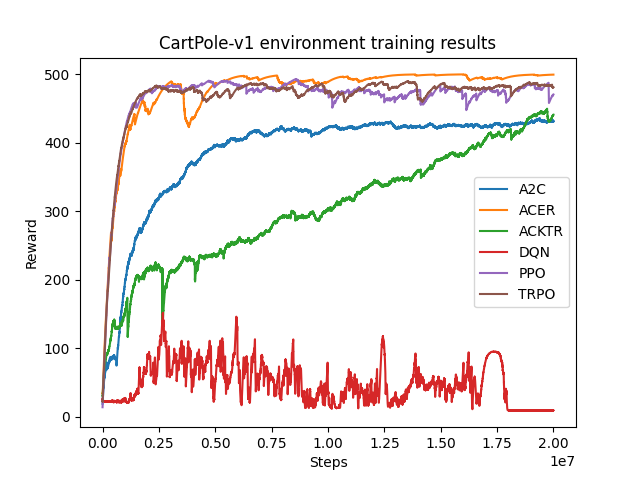
\includegraphics[width=1\linewidth]{images/cartpole_results.png}
    \caption{Discrete action space algorithms average reward}
    \label{DiscreteRewardsGraph}
\end{figure}

Since 500 is the maximum reward value for CartPole-v1 environment, most of the algorithms reached very close values at the end of training except DQN. Even after repeated trainings to check if that was not just unlucky training, it still converged to near 0 values. It seems, at least without hard tweaking of hyperparameters, DQN is the worst choice for discrete action space environments. 

If best final result is the most important aspect for your algorithm, ACER would be the obvious choice, reaching average reward of 499.528 in the end. PPO and TRPO are close second with average reward of ~475 (470.529 and 481.052 respectively), while A2C and ACKTR are a bit lower with rewards of 431.022 and 441.254. However, from analyzing its learning curve, ACKTR might reach higher rewards if training time were longer, since it was steadily going upwards all of the training time.

After analyzing training speed until algorithms converged, results were as shown in Figure \ref{DiscreteSpeedGraph}.
\begin{figure}[H]
    \centering
    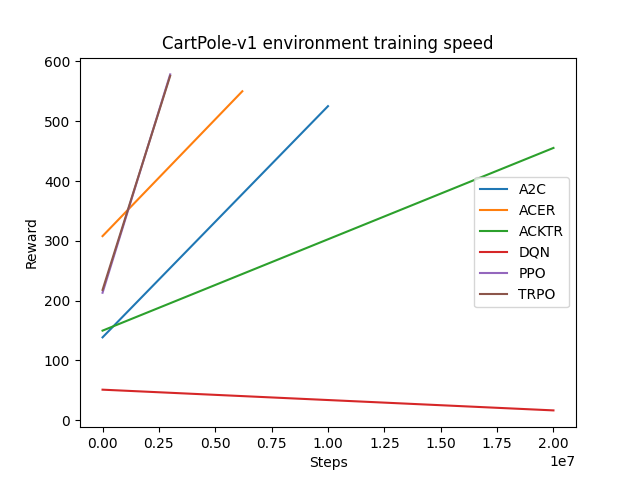
\includegraphics[width=1\linewidth]{images/cartpole_results_speed.png}
    \caption{Discrete action space algorithms training speed visualization}
    \label{DiscreteSpeedGraph}
\end{figure}

Each linear function can be represented as y=ax+b. In this case, variable "a" represents training speed and "b" represents reward at the beginning of training. 

It is clear that PPO and TRPO improved the fastest (training speed of 1.127e-4 and 1.193e-4 respectively) and even though ACER had highest average reward at the end, it had to go through some ups and downs to reach that (training speed 3.906e-5), wihch is very similar to A2C (3.866e-5). As previously mentioned, ACKTR was improving through all of the training and had not converged, so its training speed is slower (1.527e-5) and DQN having completely failed this training, have negative training speed.

If training time is limited, one might consider short term results to determine algorithm efficiency, however, similar to final results, ACER is at the top and PPO and TRPO is close second when compared average rewards at the start or very close to the start (b values of 307.869, 213.154, 217.923 respectively).

\subsection{Experiments in continuous space}

After training all algorithms, which support continuous space, results were as show in Figure \ref{ContinuousRewardGraph}. 
\begin{figure}[H]
    \centering
    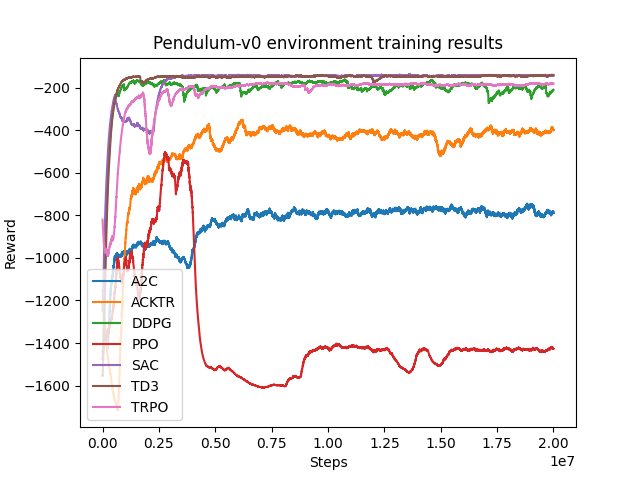
\includegraphics[width=1\linewidth]{images/pendulum_results.png}
    \caption{Continuous action space algorithms average reward}
    \label{ContinuousRewardGraph}
\end{figure}

Pendulum environment does not have maximum episode reward, however maximum single step reward is 0\footnote{https://github.com/openai/gym/wiki/Pendulum-v0}. That makes theoretical maximum episode reward 0, however, it is impossible, since pendulum starts at random position, not at the top instantly. Maximum achieved average reward is $-123.11 \pm 6.86$\footnote{https://github.com/msinto93/D4PG}.

TD3 and SAC performed insanely well with average reward scores at the end of -138.925 and -143.459. TRPO and DDPG were close behind with -181.805 and -209.935. ACKTR and A2C converged to relatively low values (-399.778, -788.661) compared to other algorithms.
Surprisingly, PPO, which performed very well in discrete action space, falls short in continuous. Even after repeated testing, it starts well and converges to a very low value near the minimum (in this case -1427.007).

After analyzing training speed until algorithms converged, results were as shown in Figure \ref{ContinuousSpeedGraph}.
\begin{figure}[H]
    \centering
    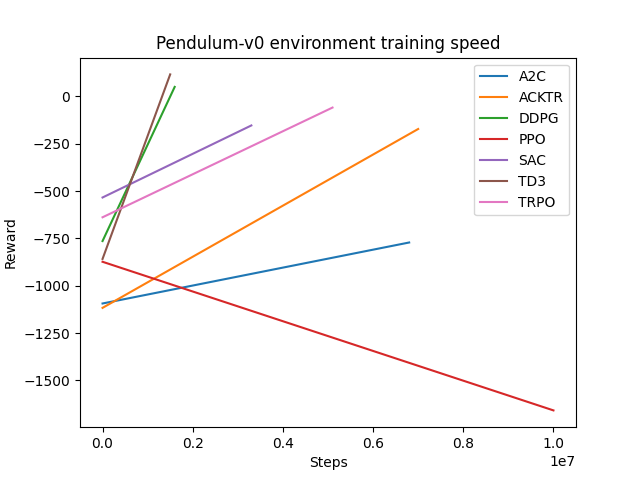
\includegraphics[width=1\linewidth]{images/pendulum_results_speed.png}
    \caption{Continuous action space algorithms training speed visualization}
    \label{ContinuousSpeedGraph}
\end{figure}

Similar to average reward scores, TD3 and DDPG are in clear lead in training speed with variable a values of 6.493e-4 and 5.085e-4. ACKTR, TRPO and SAC have a quite lower speed but consistent between the 3 of them (1.349e-4, 1.136e-4, 1.152e-4). Even though A2C converged into quite low value, it still took a while and its speed is only 4.735e-5. As previously seen, PPO underperformed and after starting well it fell down, thus its the only algorithm with negative training speed (-7.844e-5).

When comparing variable b (reward at the beginning of training), there aren't very obvious outliers. SAC is in the lead with -534.159, then goes TRPO with -638.668, DDPG with -764.094, TD3 with -858.494, PPO with -873.448, A2C with -1093.634 and ACKTR with -1116.712.

\subsection{Experiments results}

Experiment showed, that by using Stable Baselines implementation of RL algorithms with default hyperparamters and MlpPolicy on OpenAI Gym discrete environment CartPole-v1, algorithm ACER got by far the best results after training for 20 million steps, however it trained a bit slower than PPO and TRPO until it converged, making them viable alternatives if training time is limited, especially that they converge into very high average reward, which is only about 5\% behind ACER. For exact values see Table \ref{DiscreteFinalTable}.

\begin{table}[H]
\centering
\begin{tabular}{|l|l|l|} 
\hline
Algorithm & Final average reward & Training speed linear function formula  \\ 
\hline
A2C       & $431.022$              & $3.866\cdot10^-5x + 138.584$                     \\
ACER      & $499.529$              & $3.906\cdot10^-5x + 307.869$                     \\
ACKTR     & $441.254$              & $1.527\cdot10^-5x + 149.826$                     \\
DQN       & $9.457$                & $-1.733\cdot10^-6x + 51.137$                     \\
PPO       & $470.529$              & $1.127\cdot10^-4x + 213.154$                     \\
TRPO      & $481.052$              & $1.193\cdot10^-4x + 217.923$                     \\
\hline
\end{tabular}
\caption{Discrete environment algorithm experiment results}
\label{DiscreteFinalTable}
\end{table}

When using Stable Baselines implementation of RL algorithms with default hyperparameters and MlpPolicy on OpenAI Gym continuous environment Pendulum-v0, TD3 and SAC have the best final average rewards and were the most consistent with them, but DDPG and TRPO were not far behind. When comparing learning speed, DDPG and TD3 takes the top spot and SAC is a lot worse, since it took a while until it converged. Based on that, it seems, that TD3 is the best choice, since it learns quickly and converges into best average reward. For exact values see Table \ref{ContinuousFinalTable}.

\begin{table}[H]
\centering
\begin{tabular}{|l|l|l|} 
\hline
Algorithm & Final average reward & Training speed linear function formula  \\ 
\hline
A2C       & $-788.661$             & $4.735\cdot10^-5x - 1093.634$                   \\
ACKTR     & $-399.778$             & $1.349\cdot10^-4x - 1116.712$                    \\
DDPG      & $-209.935$             & $5.085\cdot10^-4x - 764.094$                     \\
PPO       & $-1427.007$            & $-7.844\cdot10^-5x - 873.448$                    \\
SAC       & $-143.459$             & $1.152\cdot10^-4x - 534.159$                     \\
TD3       & $-138.925$             & $6.493\cdot10^-4x - 858.494$                     \\
TRPO      & $-181.805$             & $1.136\cdot10^-4x - 638.668$                     \\
\hline
\end{tabular}
\caption{Continuous environment algorithm experiment results}
\label{ContinuousFinalTable}
\end{table}

\section*{Conclusions}

After completing experiments and analyzing their results, author concludes, that choosing an appropriate RL algorithm is important, since that can drastically change the result and quality of the end product. 

When choosing an algorithm, the most important factors are final average reward and training speed, which greatly differs depending on algorithm and environment action space combination:
\begin{itemize}
  \item With discrete action space, ACER algorithm greatly outperformed its competitors with almost perfect average reward, albeit a bit slower learning speed. If learning speed is more important, one might consider using PPO or TRPO as they trained much quicker than ACER but didn't reach as high final result. Other algorithms were much worse in both aspects, however, it should be noted that ACKTR never converged and its potential final result could be higher given enough training time.
  \item With continuous action space, TD3 and SAC have every other algorithm beat in final average reward, but SAC falls on in training speed to DDPG, which is also quite close to TD3 and SAC final reward results. Considering that, TD3 is the best algorithm to use on continuous actions spaces based on these results. Other algorithms falls short of previously mentioned ones with poor learning speed and converging on quite lower average rewards. 
\end{itemize}

\newpage

\bibliographystyle{alpha}
\bibliography{sources}

\end{document}